\documentclass[12pt]{article}
\usepackage[top=0.5in, bottom=0.8in, left=0.5in, right=0.5in]{geometry}

\usepackage{amsmath,amssymb,amsfonts,amsthm}
\usepackage[english]{babel}
\usepackage[T1]{fontenc}
\usepackage{bm}
\usepackage{verbatim}
\usepackage[all]{xy}
\usepackage[pdftex]{hyperref}
\usepackage{graphicx}
\graphicspath{ {./} }
\hypersetup{colorlinks=false, linkcolor=blue, pdffitwindow=true, pdftitle={Modified Model I}}

\title{Modified Model I}
\author{Wei Cui}
\begin{document}
\maketitle
\section{Observation 1}

In the original model, the solution of ODE
\begin{equation}
D\frac{d^{2}R}{dx^2} = k_{nf}R - k_{pf}R^{\alpha}\(1 - \frac{\int_{-L}^{L}Rdx}{R_{tot} }\)
\end{equation}
increases on $[-L, 0]$ and decreases on $[0, L]$. But the data is not always like this. 

\begin{figure}[h]
\caption{A Typical Sample of data}
\label{fig:sample}
\centering
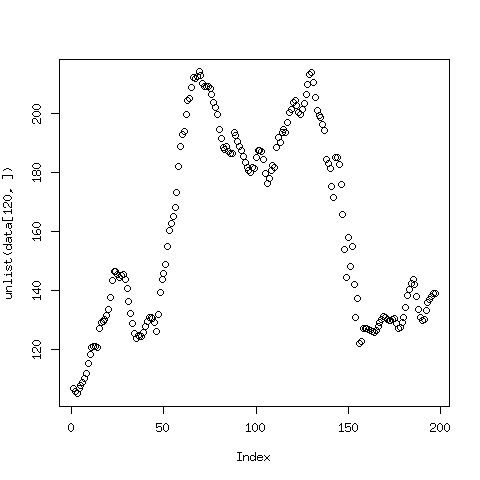
\includegraphics{sample}
\end{figure}

There is a reasonable explanation of this phenomenon. With the growth of pollen tube in this specific direction, new molecules generate on membrane which pulls down the density of ROP1 of the growth center. With this explanation we may keep the dynamic system and only adjust the measurement system.  
\section{Observation 2}


\end{document}
